\documentclass{article}[12pt, letterpaper]
% Paquetes
\usepackage{graphicx}
\usepackage{amsmath}
% %%%%%
\title{Documento 1 de Latex Laboratorio 1}
\author{D. Lara 17002265}
\date{\today}

\begin{document}
	\maketitle
	Mi primer archivo de Latex para Laboratorio 1 Proc Img 2 2022
	
	\section{Entropía} 

	Se puede entender como el número de microestados equivalentes para un mismo macroestado de un sistema. Es decir, de cuántas formas posibles se pueden colocar los elementos para que el observador pueda medir macroscópicamente lo mismo.\\ % breakline	
	
	Visto de otro modo, la entropía mide la probabilidad de encontrar un estado debido a la multiplicidad de combinaciones que dan un mismo resultado.
	
	\section{\textit{Ecuacion de Entropia}}
	$S = K\ln(\omega)$.	\\ % breakline
	
	Donde:
	\begin{itemize} 
		\item S = Entropia.
		\item K = Constante de Boltzmann
		\item $\omega$ = Numero de microestados que tienen la misma probabilidad de ocurrencia
	
		
	\end{itemize}
	
	\section{\textit{El Git Log}}
	
	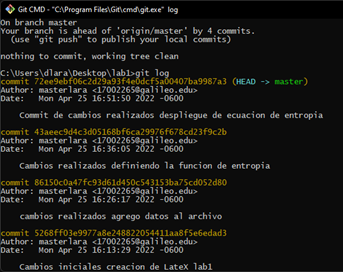
\includegraphics{log_git_ss}
	
\end{document}
